\documentclass{beamer}
\usepackage[T2A]{fontenc}
\usepackage[utf8]{inputenc}
\usepackage[english, russian]{babel}
\usepackage{graphicx, mathtools}
\graphicspath{{images/}}

\usetheme{Madrid}
\usecolortheme{default}

\title{О функции Миттаг-Леффлера и её приложениях в теории дифференциальных уравнений в дробных производных}
\date{25.06.2021}
\author{\textbf{Обучающаяся:} Тарасова Екатерина Сергеевна\\\textbf{Руководитель:} д. ф.-м. н., проф. Каменский Михаил Игоревич}

\setbeamertemplate{frametitle}[default][center]
\setbeamertemplate{navigation symbols}{}
\setbeamertemplate{footline}[page number]
\setbeamertemplate{caption}[numbered]

\DeclarePairedDelimiter{\norm}{\lVert}{\rVert}

\begin{document}

    \frame{\titlepage}

    \begin{frame}
        \frametitle{Постановка задачи}
        В данной работе ставятся и решаются следующие задачи:
        \begin{enumerate}
            \item Найти условие разрешимости задачи (\refeq{eq:cd_0q});
            \item Обосновать возможность применения метода теории степени уплотняющих отображений;
            \item Найти графический вид функции, являющейся априорной оценкой решений.
        \end{enumerate}
    \end{frame}

    \begin{frame}
        \frametitle{Задача Коши для полулинейного дифференциального включения дробного порядка}
        Рассмотрим задачу Коши для полулинейного дифференциального включения дробного порядка в $H$:

        \begin{equation}
            \label{eq:cd_0q}
            {}^CD_{0}^{q}x(t) \in Ax(t) + F(t, x(t)), \quad t \in [0, T]
        \end{equation}

        \begin{equation}
            \label{eq:cd_0q_x0}
            x(0) = x_0,
        \end{equation}

        \noindent где $0 < q < 1$ и линейный оператор $A$ удовлетворяет следующему условию:
        (A) $A: D(A) \subseteq H \rightarrow H$ - линейный замкнутый (не обязательно ограниченный) оператор, порождающий ограниченную $C_0$-полугруппу
        ${U_A(t)}_{t \geq 0}$ линейных операторов в $H$ и такой, что

        \begin{equation*}
            \langle Ax, x \rangle \leq -d \norm{x}^2, \forall x \in D(A)
        \end{equation*}

        \noindent для некоторых $d > 0$.
    \end{frame}

    \begin{frame}
        \frametitle{F}
        $F: [0, T] \times H \rightarrow K_v(H)$ - мультиотображение, основным свойством которого является:
        \begin{equation*}
            \begin{gathered}
                \exists \  a \geq 0 \  \text{такое, что}\\
                \sup_{y \in F(t,x)} \langle y,x \rangle \leq a \norm{x}^2 + G(t), \quad t \in [0, T]
            \end{gathered}
        \end{equation*}
    \end{frame}

    \begin{frame}
        \frametitle{Теорема о существовании априорной оценки}
        \textbf{Теорема:}
        При указанных выше условиях существует непрерывная функция $C: [0, +\infty) \rightarrow [0, +\infty)$ такая,
        что для любого решения $x$ задачи (\ref{eq:cd_0q})-(\ref{eq:cd_0q_x0}), определенного на интервале $[0, T]$,
        справедлива следующая априорная оценка:
        $$\norm{x}_{C([0, T], H)} \leq \mathcal{C}(T).$$

        \textbf{Теорема:}
        При указанных выше условиях задача (\ref{eq:cd_0q})-(\ref{eq:cd_0q_x0}) имеет слабое решение на $[0, T]$ для каждого $T > 0$.
    \end{frame}

    \begin{frame}
        \frametitle{Функция априорной оценки}
        Функция априорной оценки $\mathcal{C}$ на интервале $[0, T]$:
        \begin{equation}
            \label{eq:C}
            \norm{x(t)}^2 \leq E_q(t)\norm{x_0} + \int_0^t (t-s)^{q-1} E_{q,q}((-d+a)(t-s)^q)G(s)ds
        \end{equation}
        где
        \begin{equation*}
            \begin{aligned}
                &E_{\alpha, \beta}(z) = \sum_{k=0}^\infty \frac{z^k}{\Gamma (\alpha k + \beta)} - \text{функция Миттаг-Леффлера,}\\
                &\Gamma(z) = \int_0^{+\infty} t^{z-1} e^{-t} dt, \quad z \in \mathbb{C}, \quad Re(z) > 0 - \text{Гамма-функция Эйлера.}
            \end{aligned}
        \end{equation*}
    \end{frame}

    \begin{frame}
        \frametitle{Программа для построения графика}
        \begin{columns}
 
            \column{0.5\textwidth}
            \begin{figure}
                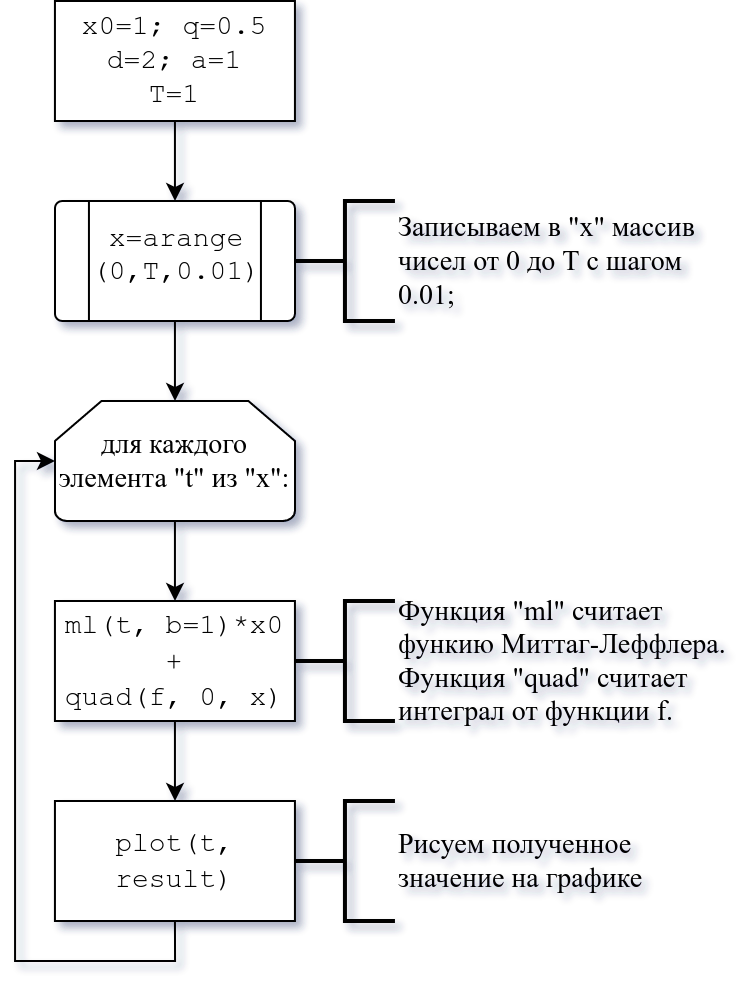
\includegraphics[width=0.8\linewidth]{diagram}
            \end{figure}
             
            \column{0.5\textwidth}
            \begin{figure}
                
\includegraphics[width=0.5\linewidth]{python-logo}
            \end{figure}
            \begin{figure}
                
\includegraphics[width=0.5\linewidth]{matplotlib-logo}
            \end{figure}
            \begin{figure}
                
\includegraphics[width=0.5\linewidth]{scipy-logo}
            \end{figure}
            \begin{figure}
                
\includegraphics[width=0.5\linewidth]{numpy-logo}
            \end{figure}

        \end{columns}
    \end{frame}

    \begin{frame}
        \frametitle{График функции априорной оценки}
        \begin{figure}
            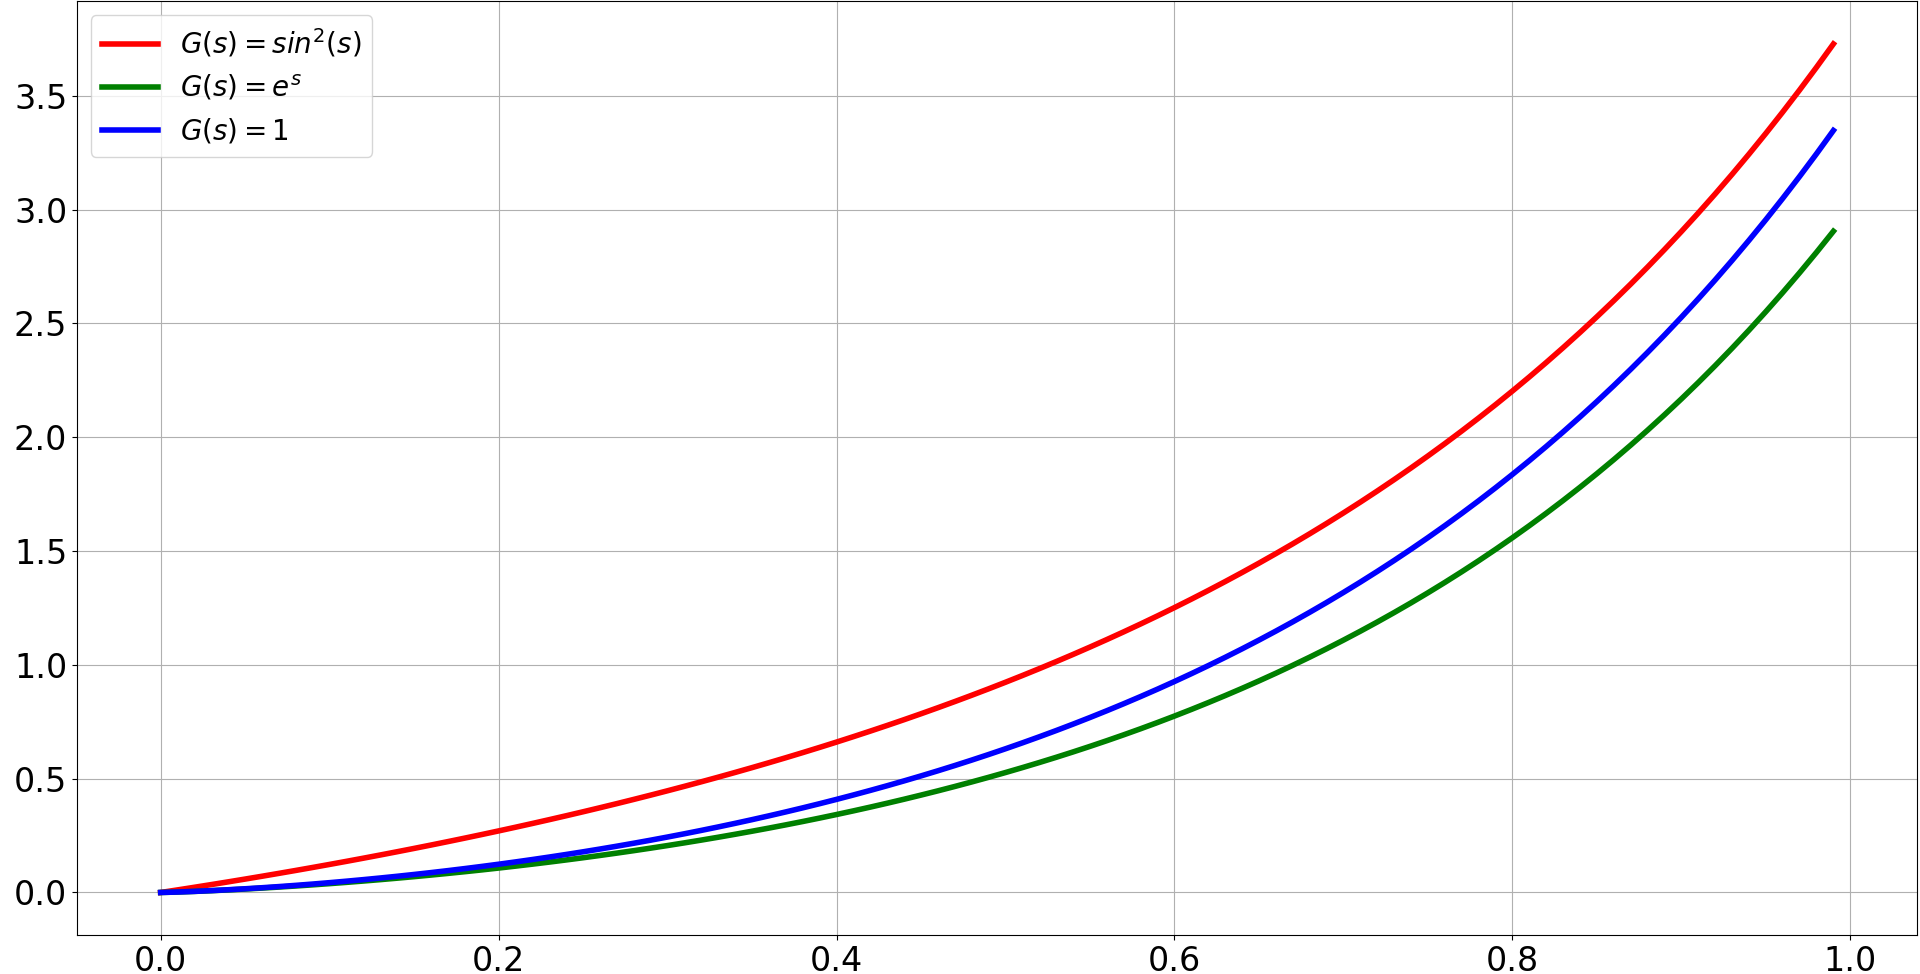
\includegraphics[width=0.75\linewidth]{plot}
            \caption{График функции (\ref{eq:C}) при $\norm{x_0} = 1$; $q = 0.5$; $d = 2$; $a = 1$; $T = 1$.}
        \end{figure}
    \end{frame}

    \begin{frame}
        \begin{block}{}
            \centerline{\color{blue}Спасибо за внимание!}
        \end{block}
    \end{frame}

\end{document}